\subsubsection{11.04.15}
\begin{enumerate}
	
	\item The time of beginning and ending of the meeting: 17:00 - 21:00.
	
	\item Purposes of the meeting: 
	\begin{enumerate}
		
		\item To make a video for the nomination "Compass Award"
		
	\end{enumerate}

	\item Work that has been done:
	\begin{enumerate}
		
		\item Today we were making a 1-minute video for the nomination "Compass Award". Thye deadline for sending video ot jidges was the following day, so we needed to shoot all the material today. That's why we didn't do anything with construction of our robot.
		
		\item Unfortunately, There were only three of us who managed to come. Our coach Dmitry Luzin and our captain Georgiy Kryliv were on "Robochallenge" competiotion in Austria (they achieved there the 2-nd place in nomination "Puck Collect"). Maksim Radionov couldn't come too. So, we made a video witout them. Although it was difficult to make a video about our coach withiut him and a half of the team, but we did our best to do it wuth a high quality.
        \begin{figure}[H]
        	\begin{minipage}[h]{0.2\linewidth}
        		\center  
        	\end{minipage}
        	\begin{minipage}[h]{0.6\linewidth}
        		\center{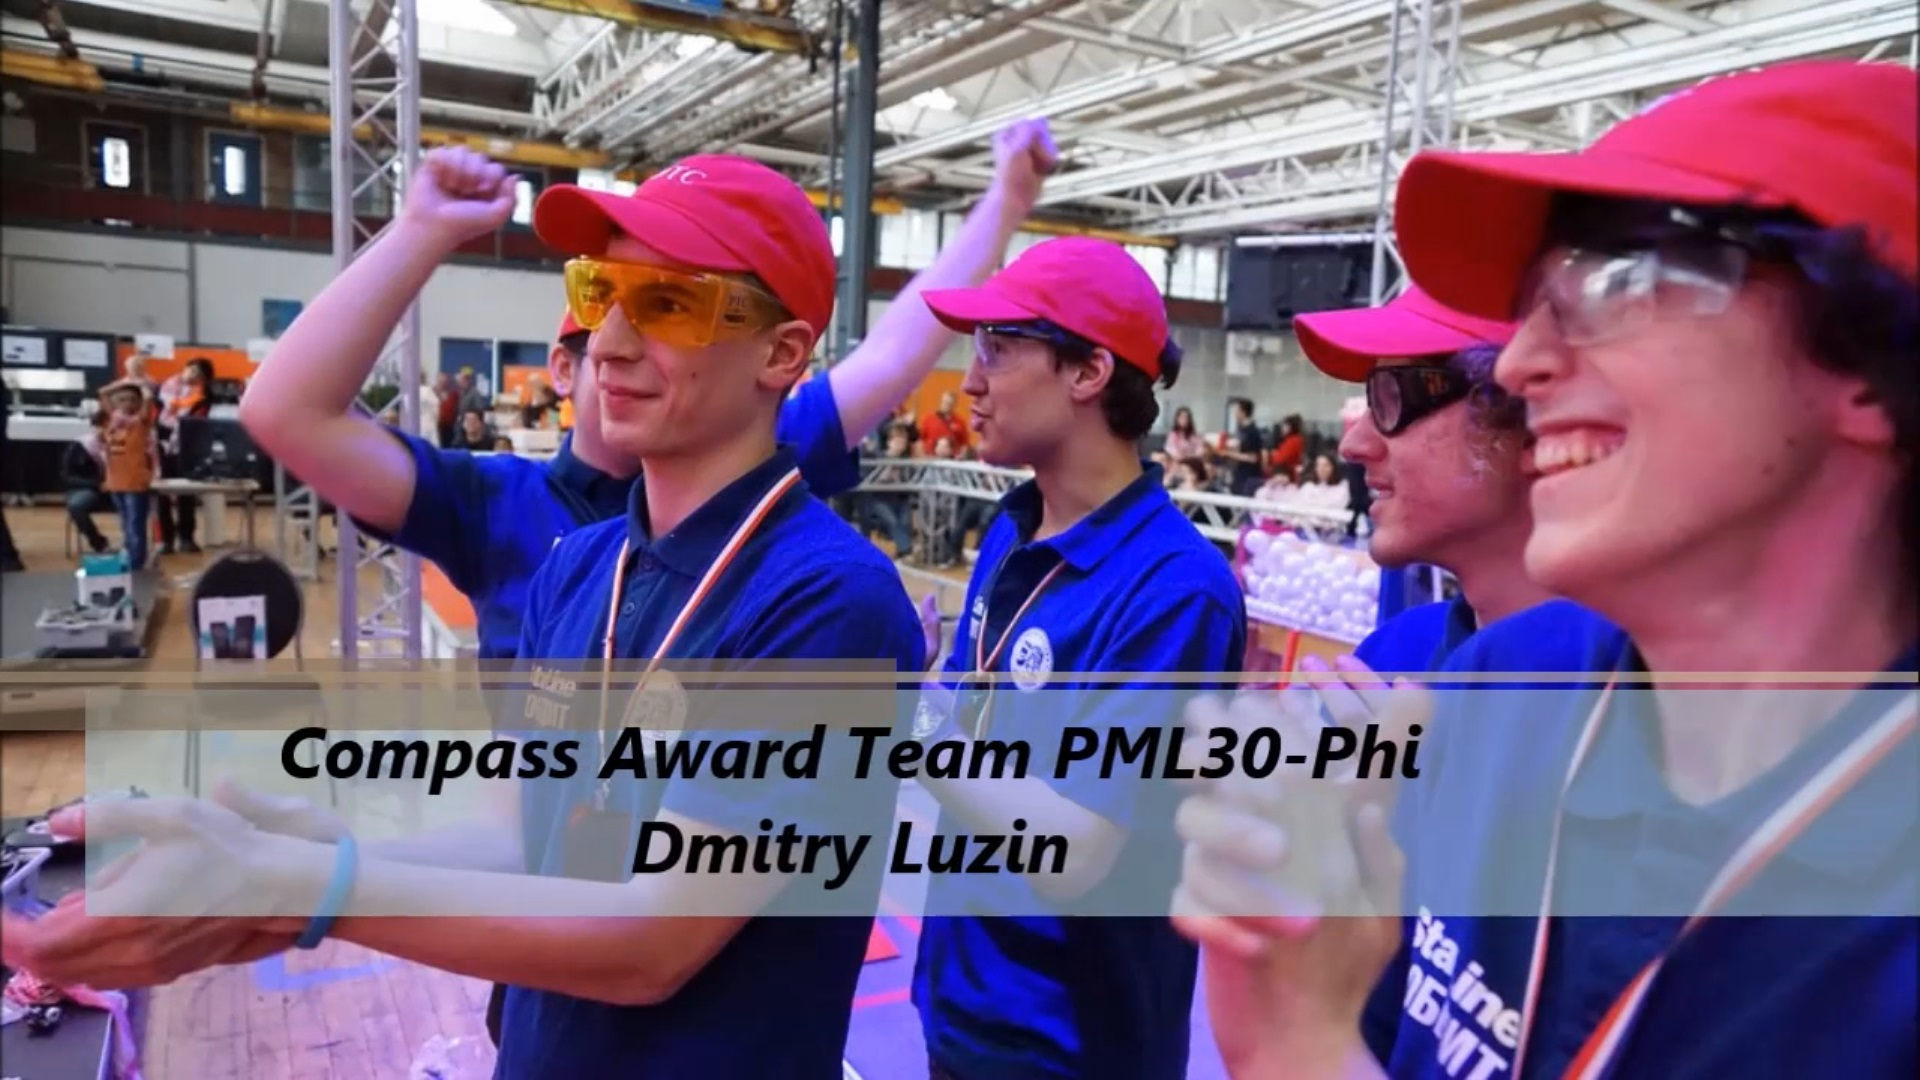
\includegraphics[scale=0.24]{days/11.04.15/images/01}}
        		\caption{The frame from our video}
        	\end{minipage}
        \end{figure}

	\end{enumerate}
	
	\item Results:
	\begin{enumerate}
		
		\item The material was shot.
		
		\item Ivan Fokin will do the video editing at home.
		
	\end{enumerate}
	
	\item Tasks for the next meetings:
	\begin{enumerate}
		
		\item Send the video to judjes.
			
	\end{enumerate}
\end{enumerate}
\fillpage
